\section{FitzHugh-Nagumoモデル}
\subsection{FitzHugh-Nagumoモデルの定義}
前節では神経活動のダイナミクスを微分方程式で表したHodgkin-Huxley(HH)モデルを扱った.HHモデルの特徴は,4変数で構成され,各変数が膜電位およびNaチャネルやKチャネルなどの活性/不活性状態を意味することである.このHHモデルをより簡易化し,2変数で神経活動の興奮とその伝播を表そうと提案されたのが\textbf{FitzHugh-Nagumo (FHN)モデル}\index{FitzHugh-Nagumo (FHN)もでる@FitzHugh-Nagumo (FHN)モデル} である.FHNモデルはvan der Pol振動子をFitzHughが修正し\citep{FitzHugh1955-bx} \citep{Fitzhugh1961-fp},南雲らによりトンネル (江崎) ダイオードを用いて電子回路上に実装\footnote{神経活動を再現する電子回路を\textbf{ニューリスタ}\index{にゅーりすた@ニューリスタ}  (neuristor) という.}された \citep{Nagumo1962-ob}という経緯がある.FHNモデルは以下で表される.
\begin{align} 
\frac{dv}{dt} &= c\left(v-\frac{v^3}{3}-u+I_e\right)\\ 
\frac{du}{dt} &= v-bu+a 
\end{align}
$v$は膜電位で,$u$は回復変数(recovery variable)と呼ばれる. FitzHughにより,HHモデルにおける$(V, m)$および$(n, h)$がそれぞれFHNモデルの$v$および$u$に対応すると説明されている \citep{Fitzhugh1961-fp} \footnote{HHモデルにおける$V$と$m$は強い正の相関があり,$n$と$h$は強い負の相関があるため,それぞれの変数の組は1つの変数に縮約されうる.}.$a,b,c$は定数であり,$a=0.7, b=0.8, c=10$がよく使われる.$I_e$は外部刺激電流に対応する.
\begin{lstlisting}[language=julia]
using Parameters: @unpack # or using UnPack
using PyPlot
rc("axes.spines", top=false, right=false)
\end{lstlisting}
変更しない定数を保持する \jl{struct} の \jl{FHNParameter} と, 変数を保持する \jl{mutable struct} の \jl{FHN} を作成する.
\begin{lstlisting}[language=julia]
abstract type Layer end
abstract type Neuron <: Layer end

@kwdef struct FHNParameter{FT}
    a::FT = 0.7; b::FT = 0.8; c::FT = 10.0
end

@kwdef mutable struct FHN{FT} <:Neuron
    num_neurons::UInt16
    dt::FT = 1e-2
    param::FHNParameter = FHNParameter{FT}()
    v::Vector{FT} = fill(-1.0, num_neurons) 
    u::Vector{FT} = zeros(num_neurons)
end
\end{lstlisting}
次に変数を更新する関数\jl{update!}を書く.ソルバーとしては陽的Euler法または4次のRunge-Kutta法を用いる.以下ではEuler法を用いている.Juliaではforループを用いて1つのニューロンごとにパラメータを更新する方がベクトルを用いるよりも高速である.
\begin{lstlisting}[language=julia]
function update!(neuron::FHN, x::Vector)
    @unpack num_neurons, dt, v, u = neuron
    @unpack a, b, c = neuron.param
    @inbounds for i = 1:num_neurons
        v[i] += dt * c * (-u[i] + v[i] - v[i]^3 / 3 + x[i])
        u[i] += dt * (v[i] - b*u[i] + a)
    end
    return v
end

(layer::Layer)(x) = update!(layer, x)
\end{lstlisting}
\subsection{FitzHugh-Nagumoモデルのシミュレーションの実行}
いくつかの定数を設定してシミュレーションを実行する.
\begin{lstlisting}[language=julia]
T = 100 # ms
dt = 0.01 # ms
nt = UInt32(T/dt) # number of timesteps
num_neurons = 1 # ニューロンの数

# 入力刺激
time = (1:nt)*dt
Ie = repeat(0.5 * ((time .> 10) - (time .> 45)) + 0.34 * ((time .> 55) - (time .> 90)), 1, num_neurons)  # injection current

# 記録用
varr, uarr = zeros(Float32, nt, num_neurons), zeros(Float32, nt, num_neurons)

# modelの定義
fhn_neurons = FHN{Float32}(num_neurons=num_neurons, dt=dt)

# simulation
@time for t = 1:nt
    v = fhn_neurons(Ie[t, :])
    varr[t, :], uarr[t, :] = v, fhn_neurons.u
end
\end{lstlisting}
結果を描画する.
\begin{lstlisting}[language=julia]
figure(figsize=(5,4))
subplot(3, 1, 1); plot(time, varr[:, 1], label=false, color="black"); ylabel("v")
subplot(3, 1, 2); plot(time, uarr[:, 1], label=false); ylabel("u"); 
subplot(3, 1, 3); plot(time, Ie, label=false); ylabel("Current"); xlabel("Times (ms)")
tight_layout()
\end{lstlisting}
\begin{figure}[ht]
	\centering
	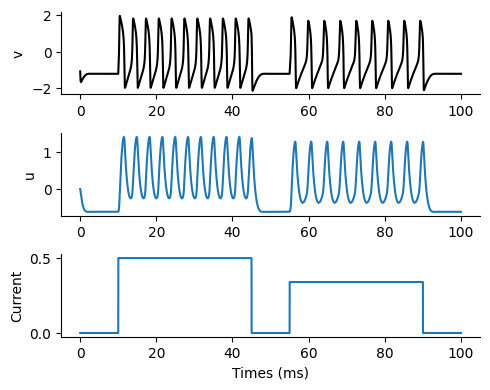
\includegraphics[scale=0.8, max width=\linewidth]{./fig/neuron-model/fhn/cell009.png}
	\caption{cell009.png}
	\label{cell009.png}
\end{figure}
\subsection{相図の描画}
phase plot
\begin{lstlisting}[language=julia]
margin = 1.0
vmax, vmin = maximum(varr) + margin, minimum(varr) - margin
umax, umin = maximum(uarr) + margin, minimum(uarr) - margin
vrange, urange = vmin:0.1:vmax, umin:0.1:umax
U = [i for i in urange, j in 1:length(vrange)]
V = [j for i in 1:length(urange), j in vrange]

a, b, c, Ie = 0.7, 0.8, 10.0, 0.34
dV = c * (-U + V - V .^3 / 3 .+ Ie)
dU = V - b*U .+ a;
\end{lstlisting}
\begin{lstlisting}[language=julia]
figure(figsize=(4,3))
streamplot(V, U, dV, dU, density=[0.8, 0.8], linewidth=2) 
contour(V, U, dU, levels=[0])
contour(V, U, dV, levels=[0])
    plot(varr, uarr); xlim(vmin, vmax); ylim(umin, umax); xlabel(L"$v$"); ylabel(L"$u$")
tight_layout()
\end{lstlisting}
\begin{figure}[ht]
	\centering
	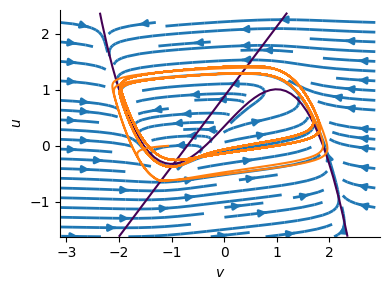
\includegraphics[scale=0.8, max width=\linewidth]{./fig/neuron-model/fhn/cell012.png}
	\caption{cell012.png}
	\label{cell012.png}
\end{figure}
